\begin{question}
\noindent A space agency designs a decorative floor emblem for its mission-control building. The emblem starts as triangle $T$ with vertices $A(1,1)$, $B(1,3)$, $C(2,1)$, shown on the grid below.

\begin{center}
\scalebox{0.75}{%
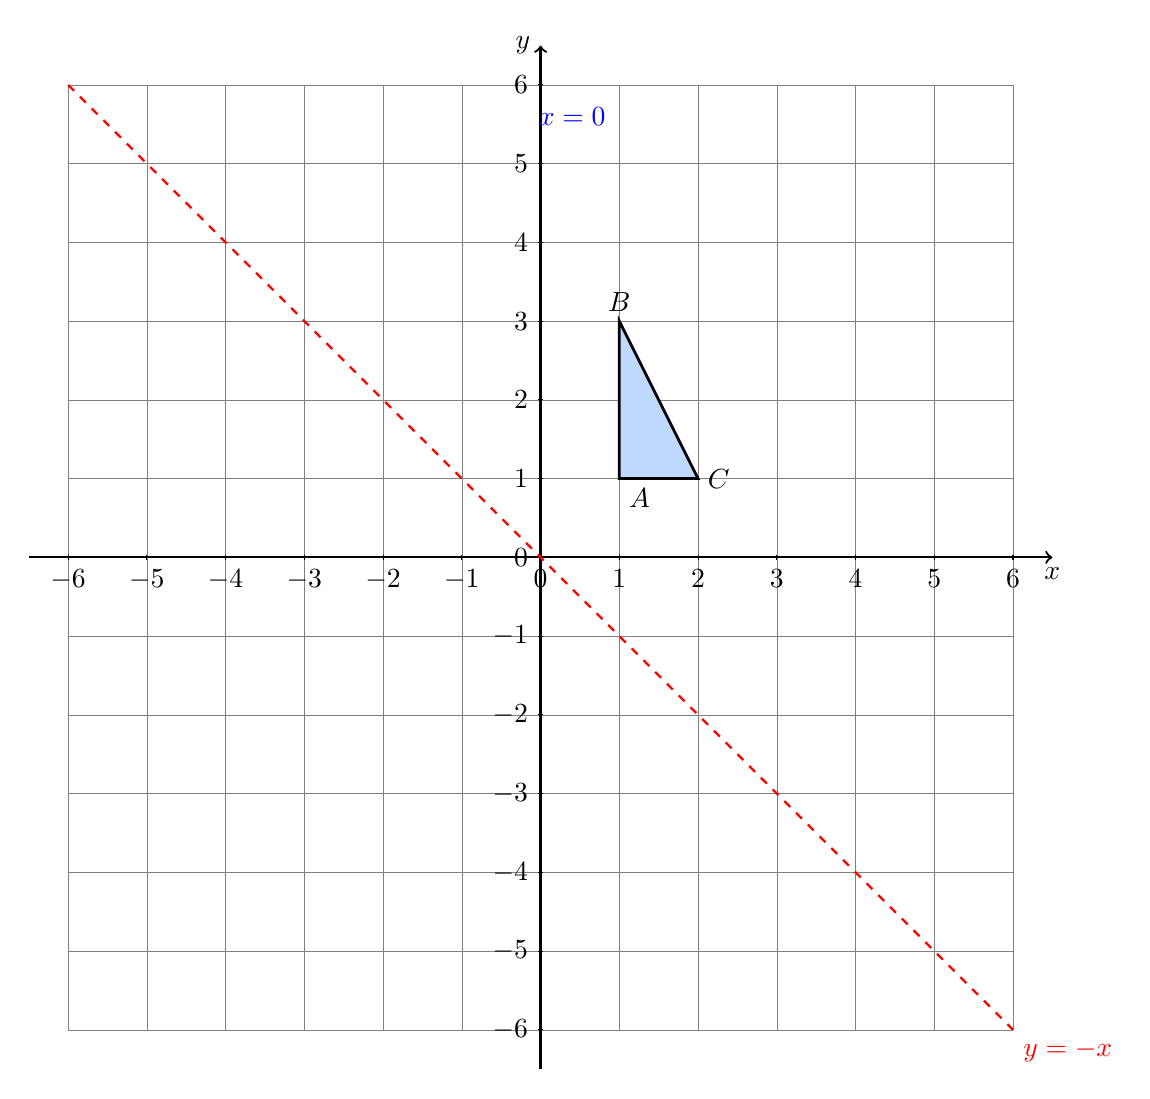
\begin{tikzpicture}
    \def\axisLimit{6}
    \definecolor{borderColour}{HTML}{000000}
    \definecolor{fillColourT}{HTML}{BFD8FF}

    % Draw grid
    \draw[step=1cm,gray,very thin] (-\axisLimit,-\axisLimit) grid (\axisLimit,\axisLimit);

    % Draw axes
    \draw[thick,->] (-\axisLimit-0.5,0) -- (\axisLimit+0.5,0) node[anchor=north] {$x$};
    \draw[thick,->] (0,-\axisLimit-0.5) -- (0,\axisLimit+0.5) node[anchor=east] {$y$};

    % Label x-axis and y-axis
    \foreach \x in {-\axisLimit,...,\axisLimit}
        \draw (\x cm,1pt) -- (\x cm,-1pt) node[anchor=north] {$\x$};
    \foreach \y in {-\axisLimit,...,\axisLimit}
        \draw (1pt,\y cm) -- (-1pt,\y cm) node[anchor=east] {$\y$};

    % Mirror lines: x = 0 (y-axis, already drawn) and y = -x
    \draw[thick, red, dashed] (-\axisLimit,\axisLimit) -- (\axisLimit,-\axisLimit) node[below right] {$y=-x$};
    \node[blue] at (0.4,5.6) {$x=0$};

    % Triangle T: A(1,1), B(1,3), C(2,1)
    \coordinate (A) at (1,1);
    \coordinate (B) at (1,3);
    \coordinate (C) at (2,1);
    \filldraw[fill=fillColourT, draw=borderColour, line width=1pt] (A) -- (B) -- (C) -- cycle;
    \node[below right] at (A) {$A$};
    \node[above] at (B) {$B$};
    \node[right] at (C) {$C$};

\end{tikzpicture}%
}
\end{center}

\begin{enumerate}
    \item[(a)] Reflect triangle $T$ in the line $x = 0$ (the $y$-axis) to give triangle $T_1$. Then reflect triangle $T_1$ in the line $y = -x$ to give triangle $T_2$.

    On a copy of the grid (or by calculating coordinates), find the coordinates of the vertices of triangle $T_2$.

    \vspace{5cm}
    \answerplain{2}

    \item[(b)] Describe \textbf{fully} the single transformation that maps triangle $T$ directly onto triangle $T_2$.

    \vspace{4cm}
    \answerlines{3}{2}
\end{enumerate}
\end{question}
